\documentclass{article}

\usepackage[utf8]{inputenc}
\usepackage[T1]{fontenc}
\usepackage{amsmath}
\usepackage{amsfonts}
\usepackage{amssymb}
\usepackage[version=4]{mhchem}
\usepackage{stmaryrd}
\usepackage{bbold}
\usepackage{graphicx}
\usepackage{adjustbox}
\usepackage{tocloft}   % For TOC formatting
\usepackage{geometry}  % For margins
\usepackage{titlesec}  % For section formatting
\usepackage{fancyhdr}
\usepackage{float}
\usepackage[stable]{footmisc}
\usepackage{hyperref}  % For clickable links in TOC (load last)
\usepackage{mdframed}  
\usepackage{listings}  



% Document styling
\geometry{margin=1in}

% Customize section formatting (option 2: let titlesec handle the label)
\titleformat{\section}
  {\normalfont\Large\bfseries} % format
  {\thesection}                % label
  {0.5em}                      % separation
  {\rule{\textwidth}{0.4pt}\vspace{0.5em}\newline} % before-code

% adding a header
\pagestyle{fancy}
\fancyhf{}
\lhead{Problem Set 2}
\rhead{Romain Fernex - Henrik Berger}
\cfoot{ \thepage}
\renewcommand{\headrulewidth}{0.8pt}

\title{Problem Set 1 - Macroeconomics}
\author{Romain Fernex - Henrik Berger}
\date{February 2025}

\begin{document}

\maketitle
\tableofcontents

\section{Literature review}
\begin{figure}[H]
    \centering
    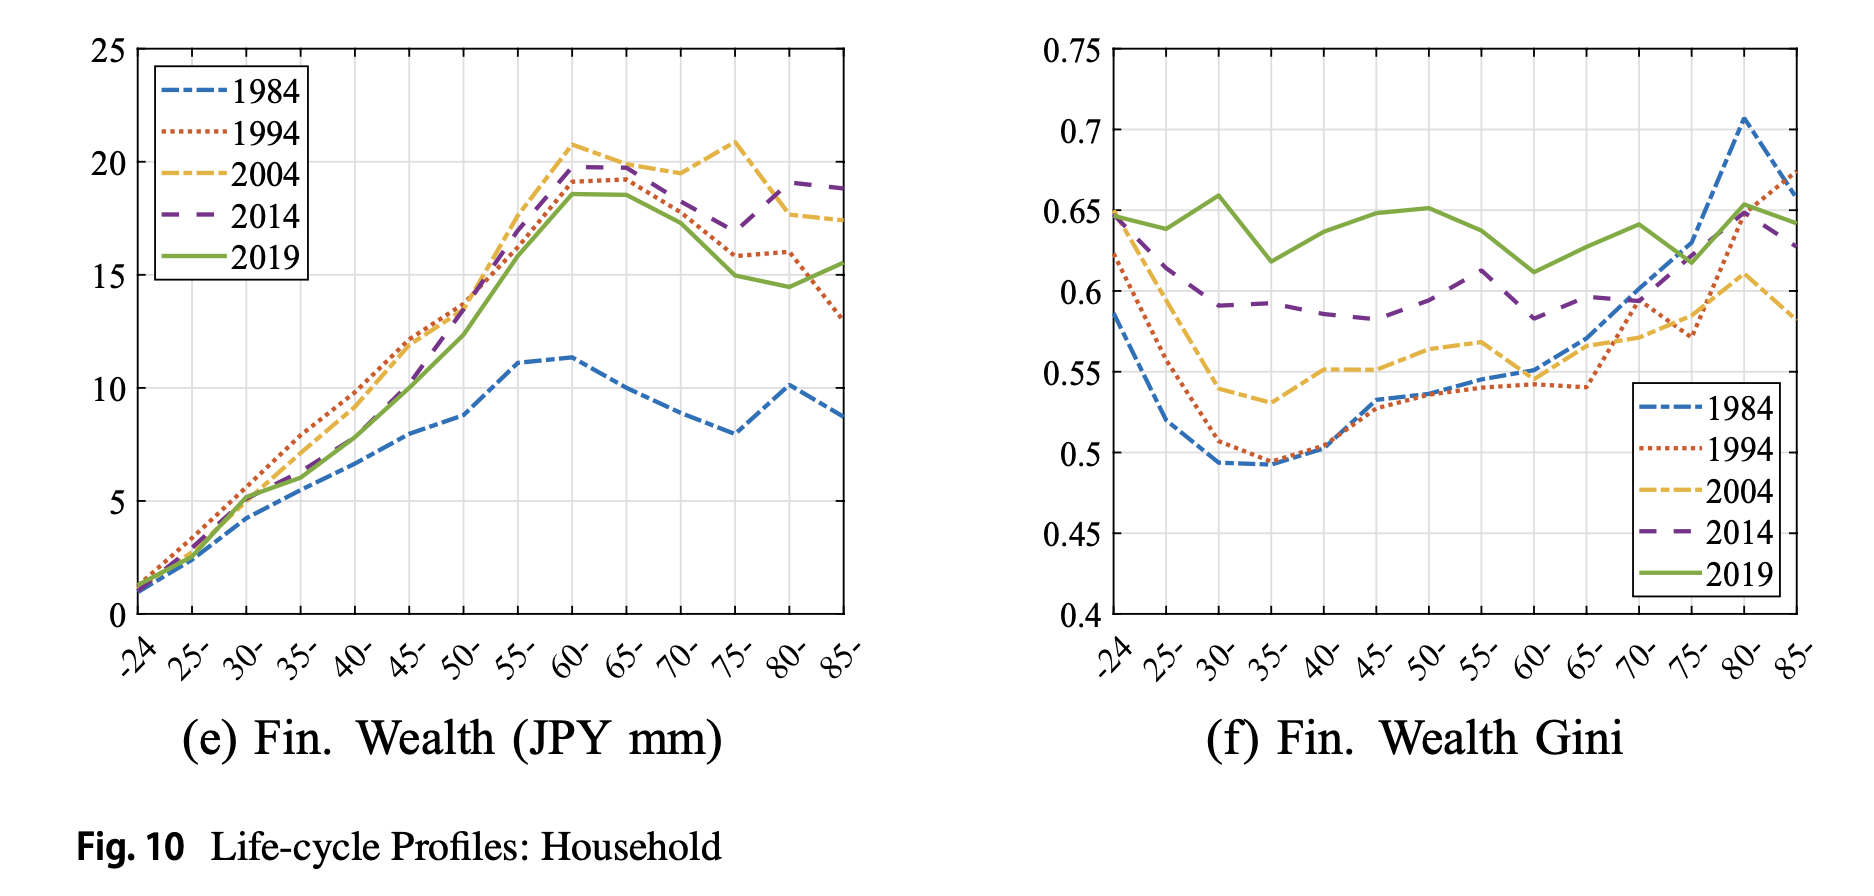
\includegraphics[width=0.8\textwidth]{figures/wealth.png}
    \caption{Comparative evolution of financial wealth levels, and of the financial wage gini coefficient between 1984 and 2019, as a function of age}
    \label{fig: Comparative evolution of financial wealth levels, and of the financial wage gini coefficient between 1984 and 2019, as a function of age}
\end{figure}
This paper describes the evolution of earnings, income, and wealth inequalities in Japan at the household level from the mid-1980s to 2019. The left-hand graph illustrates the trajectory of financial wealth among Japanese adults by age cohort. A substantial increase in financial wealth is evident for individuals aged 40 and above between 1984 and 2004, though this growth was partially dampened by the 2008 financial crisis. Younger demographics experienced a similar but considerably more modest upward trend. The right-hand graph depicts the evolution of the financial wealth Gini coefficient across age groups. Notably, while the financial wealth levels of 30-40 year-old Japanese remained relatively stable after 1994, the Gini coefficient for this cohort surged by approximately 0.13 points. Conversely, the age groups (50-70yo) who experienced the most important rise in financial wealth since the 1980s faced a more moderate gini coefficient increase (~+0.8).   Thus, while the strength of the gini coefficient was negatively correlated with age for those aged 30 and above until 1994, the heterogeneous evolution of the gini coefficient after 1994 led a marked decrease of the relation between age and inequality levels. This points to an ambiguous effect of the asset price bubble collapse of the 1990s which seems to have been associated with both an increase in financial wealth across cohorts and a leveling up of wealth inequalities for all age groups, save for senior Japanese. 


\section{Exercise I}

\subsection{1)}
The problem : $k_0$ given and $k_t,c_t \geq 0$
$$\max_{\{k_t,c_t\}_0^\infty}\sum_{t=0}^\infty\beta^t log(c_t) \hspace{0.5cm}\text{s.t } c_t+k_{t+1}\leq \theta k_t^\alpha$$
At the optimum, $c_t + k_{t+1}=\theta k_t^\alpha$
Hence the problem is : 
$$\max_{\{k_t\}_0^\infty}\sum_{t=0}^\infty\beta^tlog(\theta k_t^\alpha - k_{t+1})$$
In recursive form, we get : $$V(k_0) = \max_{0\leq k' \leq \theta k'^\alpha }\{log(\theta k ^\alpha - k') + \beta V(k')\}$$
We denote the feasibility set $\Gamma(k') = [0; \theta k^\alpha]$ for k'. k is a state variable, k' is a control varaible. 

\subsection{2)}
The FOC yields, with respect to k' : $$\begin{aligned}\frac{-1}{\theta k^\alpha-k'} + \beta V'(k') = 0 &\Longleftrightarrow \beta (\theta k^\alpha-k')V'(k') = 1\\
&\Longleftrightarrow \beta V'(k') = \frac{1}{\theta k^\alpha-k'}\end{aligned}$$
The envelope theorem yields the condition : 
$$V'(k) = \frac{\theta \alpha k^{\alpha-1}}{\theta k^\alpha-k'}$$
Hence, $V'(k') = \frac{\theta \alpha k'^{\alpha-1}}{\theta k'^\alpha-k''}$
Thus we derive the Euler equation : 
$$\beta \frac{\theta\alpha k'^{\alpha-1)}}{\theta k'^\alpha-k''}=\frac{1}{\theta k^\alpha - k'}\Longleftrightarrow \alpha\beta\theta k'^{\alpha -1}= \frac{\theta k'^\alpha -k''}{\theta k^\alpha - k'}$$

\subsection{3)}
\subsubsection{a)}
We guess that $\forall x\in \Gamma, V_0(x) = 0$. We have :
$$\begin{aligned}V_1(k) = TV_0(k) &= \max _{k'\in \Gamma(k)} log(\theta k^\alpha-k')+\beta \underbrace{V_0(k')}_{=0}\\
&= log(\theta k^\alpha)\end{aligned}$$
\subsubsection{b)}
We get : $$V_2(k) = TV_1(k) = \max_{k'\in \Gamma (k)}log(\theta k^\alpha-k')+\beta\underbrace{log(\theta k'^\alpha)}_{=V_1(k')}$$
Let $f(k') = log(\theta k^\alpha-l') + \beta log(\theta k'^\alpha)$. We derive its FOC with respect to $k'$ : 
$$\begin{aligned}
    f'(k) = \frac{-1}{\theta k^\alpha-k'}+\frac{\beta \alpha}{k'} &= 0 \\
    \Longleftrightarrow k' &= \alpha \beta(\theta k^\alpha-k') \\
    \Longleftrightarrow (1+\alpha\beta)k' &= \alpha\beta\theta k^\alpha\\
    \Longleftrightarrow k' &= \underbrace{\frac{\alpha\beta}{1+\alpha\beta}}_{\leq 1}\theta k^\alpha \leq \theta k^\alpha 
\end{aligned}$$
Thus, we have found the optimal $k'$, so : 
$$\begin{aligned}
    V_2(k) &= log(\theta k^\alpha - \frac{\alpha\beta}{1+\alpha\beta}\theta k^\alpha) + \beta log([\frac{\theta \beta\alpha k^\alpha}{1+\beta\alpha}]^\alpha)+\beta log(\theta)\\
    &= log(\frac{1}{1+\alpha\beta})+\alpha\beta log(\frac{\theta\beta\alpha k^\alpha}{1+\beta\alpha})+\beta log(\theta)\\
    &= \alpha (1+\alpha\beta)log(k) +[(1+\beta+\alpha\beta)log(\theta)+\alpha\beta log(\alpha\beta)-(1+\alpha\beta)log(1+\alpha\beta)]
\end{aligned}$$

\subsection{4)}
Let's now assume $V(k) = a_1+a_2log(k)$, we have : $$a_1+a_2log(k) = \max_{k'\in\Gamma(k)}log(\theta k^\alpha-k')+\beta (a_1+a_2log(k')) $$
Let $g(k') = log(\theta k^\alpha-k') + a_1\beta +a_2\beta log(k')$
We have : $$\begin{aligned}g'(k') = 0 &\Longleftrightarrow \frac{1}{\theta k^\alpha -k'}= \frac{a_2\beta}{k'}\\
&\Longleftrightarrow k'=\theta\beta a_2 k^\alpha-a_2\beta k'\\
&\Longleftrightarrow k' = \frac{\theta \beta a_2}{1+a_2\beta}k^\alpha
\end{aligned}$$
So we get : 
$$\begin{aligned}
    a_1+a_2log(k) &= log(\theta k^\alpha(1-\frac{a_2\beta}{1+a_2\beta})) + a_1\beta + a_2\beta log(\theta k^\alpha\frac{\beta a_2}{1+a_2\beta}) \\
    &= log(\theta\frac{1}{1+a_2\beta}) + \alpha log(k) + a_1\beta + a_2 \beta log(\theta \frac{\theta a_2\beta}{1+a_2\beta })+\alpha a_2\beta log(k)
\end{aligned}$$
Hence we get : 
$$a_2 = \alpha +\alpha a_2\beta \Longleftrightarrow a_2 = \frac{\alpha}{1-\alpha\beta}$$
Then, we find $a_1$ : 
$$\begin{aligned}
    a_1 &= a_1\beta +log(\frac{\theta }{1+\frac{\alpha \beta}{1-\alpha\beta}})+\frac{\alpha\beta}{1-\alpha\beta}log(\theta \frac{\frac{\alpha\beta}{1-\alpha\beta}}{1+\frac{\alpha\beta}{1-\alpha\beta}})\\
    \Longleftrightarrow a_1(1-\beta) &= log(\theta(1-\alpha\beta)) + \frac{\alpha\beta}{1-\alpha\beta}log(\theta\alpha\beta)\\
    \Longleftrightarrow a_1 &= \frac{1}{1-\beta}[log(\theta (1-\alpha\beta))+\frac{\alpha\beta}{1-\alpha\beta}log(\theta\alpha\beta)]
\end{aligned}$$
\subsection{5)}
Let's find the policy functions : Based on (4) we get : 
$$\begin{aligned}k' &= \frac{\beta a_2\theta k^\alpha }{1+\beta a_2}\\
&= \frac{\beta (\frac{\alpha}{1-\beta\alpha})\theta k^\alpha}{1+\beta(\frac{\alpha}{1-\alpha\beta})}\\
&= \beta\alpha\theta k^\alpha 
\end{aligned}$$
So we have : $$k' = \beta \alpha\theta k^\alpha \equiv g_k'(k)$$
Similarly, we get the policy function for c : 
$$c = \theta k^\alpha -k' = \theta k^\alpha - \beta\alpha\theta k^\alpha = (1-\beta\alpha)\theta k^\alpha \equiv g_c(k)$$
\subsection{6)}
Let us take $k_0 = 1, \alpha = \frac{1}{2}, \beta = 0.9, \theta =2$, the we get : 
$$\begin{aligned}
    k_1 &= 0.9\\
    k_2 &= \frac{9}{10}\times \frac{9}{10}^{1/2} \approx 0.854\\
    k_3 &= \frac{9}{10}^{5/2} \approx 0.768
\end{aligned}$$
And for the consumption path we get : 
$$\begin{aligned}
    c_0 &= \theta k_0^\alpha-k_1 = 2-0.9 = 1.1\\
    c_1 &= \theta k_1 ^\alpha -k_2 = 2\times 0.9^{1/2}-0.854 \approx 1.0436\\
    c_2 &= \theta k_2^\alpha -k_3 \approx 0.985
\end{aligned}$$

\section{Exercise 2}
\subsection{1)}
\begin{itemize}
    \item We assume that housing goods can be purchased at each period t for the corresponding price $P_t$. Household take the latter as granted. Purchased housing goods then depreciate at rate $\delta$ and can be sold at the price $P_t$ to acquire additional resources. 
    \item it is assumed that there is no market friction p : 1- the agent has perfect information about the price of housing goods in every period) and full ownership of the good is transferred instantaneously (can sell it back at price $P_t$ at the next period, accounting for depreciation).
\end{itemize}
\subsection{2)}
To avoid Ponzi schemes, we need to impose the following transversality condition on the financial asset $b_t$ : 
$$\lim_{t\xrightarrow{}+\infty}\beta^tb_t \geq 0 $$
Similarly, for the amount of housing good $H_t$, we need : 
$$\lim_{t\xrightarrow{}+\infty}\beta^tP_tH_t \geq 0 $$
\subsection{3)}
Let us assume that $P_t$, $y_t$ and $r_t$ are parameters and are determined exogenously at each period. Households choose how much of the housing good $H_t$ they wish to invest in, how much they wish to consume now $c_t$ and how much they wish to save for the next period through the financial asset $b_t$. The choice of the control variables $c_t,H_t,b_t$ at each period depends on parameters and on the available stock of housing goods $H_{t-1}$ and financial assets $b_{t-1}$.\\
Now that we have identified the state and control variable, we can write the value function through the Bellman equation : 
$$V(b_{-1},H_{-1}) = \max _{H,b}u(y+(1-r_{-1})b_{-1}+P(1-\delta)H_{-1}-b-PH,H) + \beta V(b,H)$$
\subsection{4)}
We begin by deriving the FOC in the control variables $H,b$ :
\begin{equation}\begin{aligned}
    &\frac{\delta V(b_{-1},H_{-1})}{\delta b} = 0 \Longleftrightarrow u_1(c,H) = \beta V_1(b,H)\\
    &\frac{\delta V(b_{-1},H_{-1})}{\delta H} = 0 \Longleftrightarrow Pu_1(c,H) - u_2(c,H) = \beta V_2(b,H)
\end{aligned}\end{equation}
Then the envelope theorem yields the following conditions in $H_{-1}, b_{-1}$ (state variables):
\begin{equation}\begin{aligned}
    &V_1(b_{-1},H_{-1}) = (1-r_{-1})u_1(c,H)\\
    &V_2(b_{-1},H_{-1}) = P(1-\delta)u_1(c,H)
\end{aligned}\end{equation}
Let's substitute (2) in (1) after evaluating the former at $(b,H)$ : 
\begin{equation}\begin{aligned}
    &u_1(c,H)  = \beta (1-r)u_1(c',H')\\
    &Pu_1(c,H) + u_2(c,H) = \beta P'(1-\delta)u_1(c',H')
\end{aligned}\end{equation}
Thus we get the Euler equations : 
\begin{equation}\begin{aligned}
  &u_1(c,H)  = \beta (1-r)u_1(c',H')\\
  &  u_2(c,H) = \beta P'(1-\delta)u_1(c',H') - Pu_1(c,H)
\end{aligned}\end{equation}

\subsection{Bonus question}
Let's use (4) to get $u_1(c',H')$ as a function of $u_1(c,H)$ :
$$u_1(c',H') = \frac{u_1(c,H)}{\beta(1-r)}$$
Now, the second equation in (4) gives us : 
$$\begin{aligned}
     u_2(c,H)&= \beta P'\frac{1-\delta}{\beta(1-r)}u_1(c,H) - Pu_1(c,H)\\
     &= (P'\frac{1-\delta}{1-r}-P)u_1(c,H)\\
\end{aligned}$$
Hence, with the notation in t, t+1 : 
\begin{equation}u_2(c_t,H_t) = (P_{t+1}\frac{1-\delta}{1-r_t}-P_t)u_1(c_t,H_t) \end{equation}
Let us compute $u_2(c_t,H_t)$ and $u_1(c_t,H_t)$ : 
$$\left\{\begin{aligned}
    &u_1(c_t,H_t) = c_t^{\rho-1}(c_t^\rho+H_t^\rho)^{\frac{1}{\rho}-1}\\
    &u_2(c_t,H_t) = H_t^{\rho-1}(c_t^\rho+H_t^\rho)^{\frac{1}{\rho}-1}
\end{aligned} \right.$$
Let's denote $U\equiv H_t^{\rho-1}(c_t^\rho+H_t^\rho)^{\frac{1}{\rho}-1}$. We substitute $u_2(c_t,H_t)$ and $u_1(c_t,H_t)$ in (5) and express $\frac{c_t}{H_t}$ as a function of other variables : 
$$\begin{aligned}
    H^{\rho-1}U &= (P_{t+1}(\frac{1-\delta}{1-r_t})-P_t)c_t^{\rho-1}U\\
    \Longleftrightarrow (\frac{c_t}{H_t})^{\rho-1} &= (P_{t+1}(\frac{1-\delta}{1-r_t})-P_t)^{-1}\\
    \Longleftrightarrow (\frac{c_t}{H_t}) &= (P_{t+1}(\frac{1-\delta}{1-r_t})-P_t)^{\frac{1}{1-\rho}}
\end{aligned}$$

\section{Exercise 3}
Please find the associated Pluto Notebook at the following link : \href{https://pluto.land/n/yguc6pup}{Notebook for Exercise 3} 

\section{Reference}
Kitao, S., Yamada, T. Earnings, income, and wealth inequality in Japan: a long-term perspective, 1984–2019. JER 76, 231–283 (2025). https://doi.org/10.1007/s42973-024-00187-0

\end{document}


